% --------------------------------------------------------------
% This is all preamble stuff that you don't have to worry about.
% Head down to where it says "Start here"
% --------------------------------------------------------------
 
\documentclass[12pt]{article}
 
\usepackage[margin=1in]{geometry} 
\usepackage{amsmath,amsthm,amssymb}
\usepackage{enumitem}
\usepackage{graphicx}
\usepackage{listings}
\usepackage{courier}
\usepackage{subcaption}

\usepackage{algorithm}
\usepackage[noend]{algpseudocode}
\algrenewcommand{\algorithmicreturn}{\State \textbf{return}}

\newcommand{\N}{\mathbb{N}}
\newcommand{\R}{\mathbb{R}}
\newcommand{\LL}{\mathcal{L}}
\newcommand{\LD}{\mathcal{L}_\mathcal{D}}
\newcommand{\LW}{\mathcal{L}_\mathcal{W}}
\newcommand{\norm}[1]{\left\lVert#1\right\rVert}

\lstset{basicstyle=\footnotesize\ttfamily,breaklines=true}

\newcommand{\irow}[1]{% inline row vector
  \begin{smallmatrix}(#1)\end{smallmatrix}%
}

\setitemize{itemsep=2pt,topsep=4pt,parsep=2pt,partopsep=2pt}
\setenumerate{itemsep=2pt,topsep=4pt,parsep=2pt,partopsep=2pt}

\newenvironment{problem}[2][Problem]{\begin{trivlist}
\item[\hskip \labelsep {\bfseries #1}\hskip \labelsep {\bfseries #2.}]}{\end{trivlist}}
\newenvironment{solution}[1][Solution]{\begin{trivlist}
\item[\hskip \labelsep {\bfseries #1.}]}{\end{trivlist}}


\begin{document}

% --------------------------------------------------------------
%                         Start here
% --------------------------------------------------------------
 
\title{ECE1513 Winter 2019 Assignment 1}
\maketitle

\begin{problem}{1}

\textbf{1.}
To facilitate computing, we extended the dimensions of both $W$ and $\mathbf{x}$ to $W'$, $\mathbf{x}'$
such that $W' = [b, W^T]^T$ and $\mathbf{x}' = [x_0 = 1, \mathbf{x}^T]^T$ to incorporate the bias term, and define
$X = [x'^{(1)T}, x'^{(2)T}, \cdots, x'^{(N)T}]$ to be the transpose of $\mathbf{x}'$.

The analytic expression for MSE can be written as:
\begin{align*}
\LL &= \LD + \LW = \sum_{n=1}^N \frac{1}{2N}\norm{W^T \mathbf{x}^{(n)} + b - y^{(n)}}_2^2 + \frac{\lambda}{2}\norm{W}_2^2\\
&= \frac{1}{2N} \sum_{n=1}^N \norm{W'^T \mathbf{x'}^{(n)} - y^{(n)}}_2^2 + \frac{\lambda}{2}\norm{W}_2^2\\
&= \frac{1}{2N} \norm{XW' - \mathbf{y}}_2^2 + \frac{\lambda}{2}\norm{W}_2^2.
\end{align*}

Now the analytical expression for the gradient can be found by:
\begin{align*}
\nabla \LL &= \nabla \frac{1}{2N} \norm{XW' - \mathbf{y}}_2^2 + \nabla \frac{\lambda}{2}\norm{W}_2^2 \\
&= \frac{1}{2N} \nabla \norm{XW' - \mathbf{y}}_2^2 + \frac{\lambda}{2} \nabla \norm{W}_2^2 \\
&= \frac{1}{2N}\big(-2 X^T\mathbf{y} + 2X^TXW'\big) + \frac{\lambda}{2}(2W) \\
&= \frac{1}{N}\big(X^TXW' - X^T\mathbf{y}\big) + \lambda W.
\end{align*}

In terms of function implementation, we also changed the function header for \texttt{MSE} and \texttt{gradMSE}, in order to accommodate for the extended dimensions of $W'$ and $\textbf{x}'$. 
Moreover, matrices multiplication is used instead of looping through the inputs. 
In the code snippet below, we use \texttt{w} to denote the weight vector $W'$, and \texttt{X} to denote
the input matrix $X$.

\begin{lstlisting}[frame=single]
def MSE(w, X, y, reg):
    N = X.shape[0]
    ld = norm_sqr(np.matmul(X, w) - y) / 2 / N
    # Use only original w for regularization
    lw = norm_sqr(w[1:]) * reg / 2
    return ld + lw
\end{lstlisting}

\begin{lstlisting}[frame=single]
def gradMSE(w, X, y, reg):
    N = X.shape[0]
    return (
        (np.matmul(np.matmul(X.T, X), w) - np.matmul(X.T, y)) / N
        + reg * np.concatenate([[0], w[1:]])
    )
\end{lstlisting}

\bigskip

\textbf{2.} The implementation of the batch Gradient Descent algorithm is carried out in the following functions:
\begin{itemize}
    \item \texttt{grad\_descent\_step}: performs one step of the Gradient Descent algorithm. It calculates the loss and the gradient in the current step using functions MSE and gradMSE from above and updates the weight. 
    \item \texttt{full\_grad\_descent}: performs the full Gradient Descent algorithm. It calls grad\_descent\_step function iteratively until the required number of epochs or the desired error tolerance is reached. It returns the optimized weight and also stores the training, validation and test losses/accuracies.   
\end{itemize}
    Refer to the source code submitted separately for detailed implementation of the functions.


\bigskip

\textbf{3.} Figure \ref{fig:1-3} plots the training, validation, and test losses of the Gradient Descent algorithm under settings $\lambda=0$, epochs=5000, $\alpha=[0.005, 0.001, 0.0001]$. As shown in the figure,  greater $\alpha$ results in faster convergence. 
\begin{figure}[!htb]
\hspace*{-2cm}
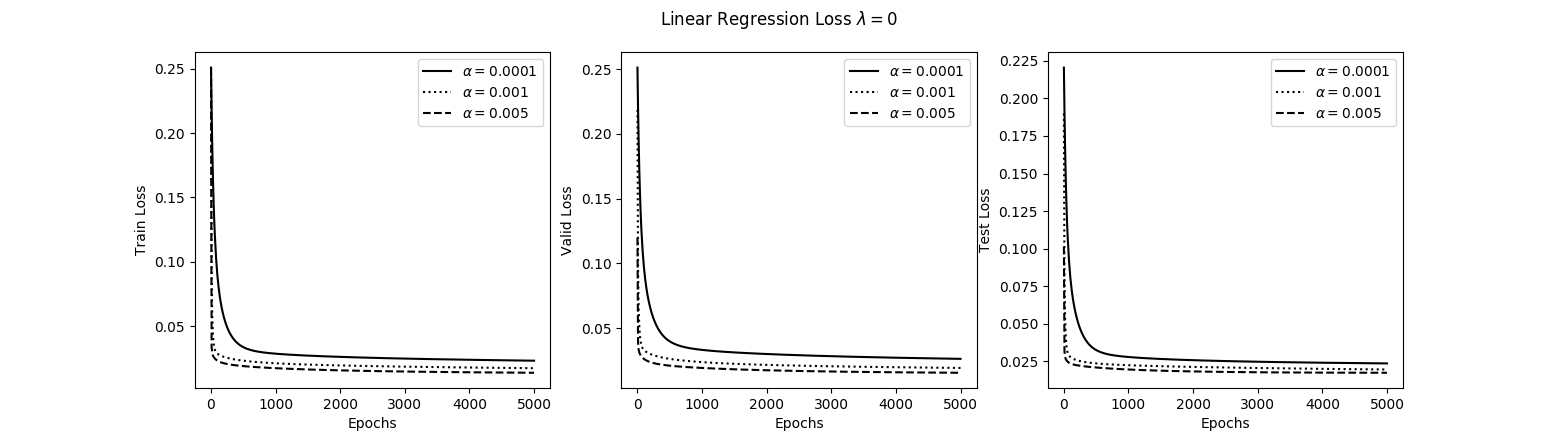
\includegraphics[width=1.2\linewidth]{images/a1/1.3/loss_all.png}
\caption{Training loss (top left), Validation loss (top right), and Test loss (bottom left) under the settings  $\lambda=0$, epochs = 5000 and $\alpha=[0.005, 0.001, 0.0001]$.}\label{fig:1-3}
\end{figure}


Table \ref{table:1-3} summarizes the final accuracy and training time with different $\alpha$ values. After 5000 epochs, greater $\alpha$ tends to achieve better accuracy on all training, validation, and test data sets. This can be considered as the consequence of faster convergence. On the other hand, the training time under different $\alpha$ settings do not appear to differ significantly, which is reasonable since all settings have to perform the same number of 5000 epochs.
\begin{table}[!htb]
\center
\begin{tabular}{rrrrr}
\hline
$\alpha$ & training accu. & validation accu. & test accu. & training time \\ \hline
0.005    & 97.89\%  & 98.00\%    & 97.24\% & 195.9s \\
0.001    & 96.31\%  & 97.00\%    & 95.86\% & 197.6s \\
0.0001   & 94.74\%  & 93.00\%    & 95.17\% & 203.1s \\ \hline
\end{tabular}
\caption{Final (epochs=5000) classification accuracy and training time with different $\alpha$ settings.}
\label{table:1-3}
\end{table}
\bigskip
\newpage
\textbf{4.} To investigate the effect of the regularization parameter $\lambda$ on the performance of the algorithm, the training, validation, and test losses under settings  $\lambda=[0.001, 0.1, 0.5]$, $\alpha=0.005$ and epochs=10000 are plotted in Figure \ref{fig:1-4} on the next page.
As shown in the figure, smaller $\lambda$ values appear to achieve lower training, validation and test losses. In the cases where $\lambda=0.5$ and $\lambda=0.1$, the training terminates after 4786 and 5145 epochs, since the error tolerence has been reached. It's worth noting that when $\lambda=0.001$, even though the training and validation losses continue to decrease, the test loss start to increase after around 5610 epochs, indicating the sign of overfitting.  


\begin{figure}[!htb]
\minipage{0.5\textwidth}
  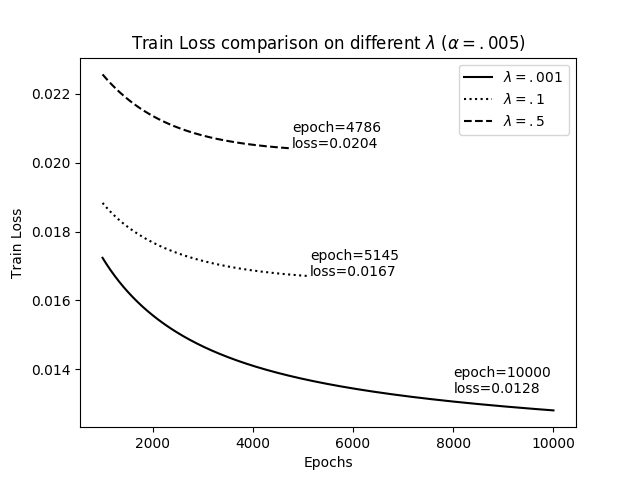
\includegraphics[width=\linewidth]{images/a1/1.4/train_loss.png}
\endminipage\hfill
\minipage{0.5\textwidth}
  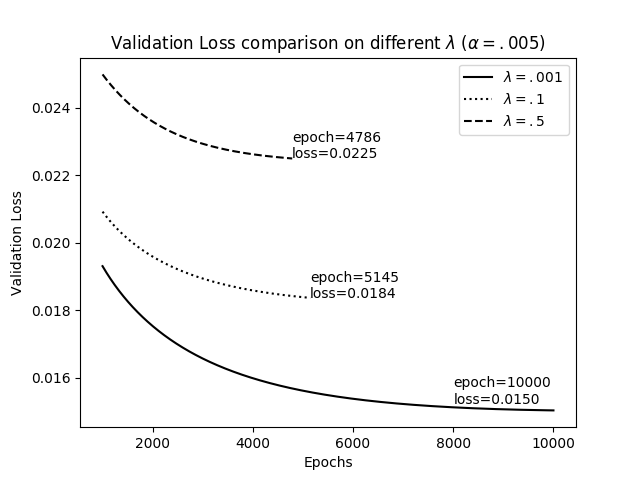
\includegraphics[width=\linewidth]{images/a1/1.4/valid_loss.png}
\endminipage\hfill
\minipage{0.5\textwidth}%
  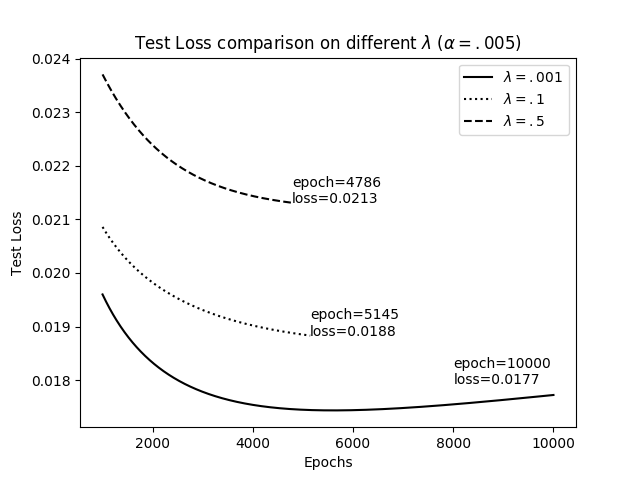
\includegraphics[width=\linewidth]{images/a1/1.4/test_loss.png}
\endminipage
\caption{Training loss (top left), Validation loss (top right), and Test loss (bottom left) under the settings  $\lambda=[0.001, 0.1, 0.5]$, $\alpha=0.005$ and epochs=10000.}\label{fig:1-4}
\end{figure}

\bigskip

Table \ref{table:1-4} summarizes the final training, validation and test accuracy using different $\lambda$ values. Choosing smaller $\lambda$ values appear to enhance final training, validation and test accuracy performance in this case. However, since the error tolerance is reached after 4786 epochs for $\lambda=0.5$ and  5145 epochs for $\lambda=0.1$, the training terminates much sooner than in the case where $\lambda=0.001$ and all 10000 epochs need to be completed. As a result, training time is greatly reduced when larger $\lambda$ values are used.


\begin{table}[!htb]
\center
\begin{tabular}{rrrrrr}
$\lambda$ & epochs & training accu. & validation accu. & test accu. & training time \\ \hline
0.001     & 10000   & 98.29\%        & 98.00\%          & 97.24\%    & 539.37s   \\
0.1       & 5145   & 97.6\%        & 97.00\%          & 96.55\%    & 269.72s   \\
0.5       & 4786   & 97.11\%        & 97.00\%          & 96.55\%    & 263.09s   \\ \hline\end{tabular}
\caption{Final classification accuracy and training time under different $\lambda$ settings. Note when $\lambda = 0.1$ and $\lambda = 0.5$, the iteration ends at 5145 and 4786 epochs respectively due to reaching the error tolerance $1\times10^{-7}$.}
\label{table:1-4}
\end{table}

\bigskip

The rationale behind tuning  $\lambda$ using the validation set is usually to prevent overfitting. As the model is trained, it may fit the training set increasingly well, but at some point start to lose its generalizability over broader data sets. The regularization parameter $\lambda$ is included into the cost function to prevent overfitting and the proper value of $\lambda$ is selected from fitting the model over the validation set.
\bigskip

\textbf{5.} The following function is written to find the optimum weights using the normal equation for the derivative of the mean square error. 

\begin{lstlisting}[frame=single]

def linear_regression_normal_equation(X, y, reg):

    """Use analytical solution of the means square error to find optimum weights
    W* = (X^T * X + \lambda * I)^-1 * X^T * Y
    """

    d = X.shape[1]
    return np.matmul(
        np.matmul(
            np.linalg.inv(
                np.matmul(X.T, X) + reg * np.eye(d)
            ),
            X.T
        ),
        y
    )
\end{lstlisting}

\bigskip

Table \ref{table:1-5} summarizes the final error, accuracy and training time of the normal equation algorithm when $\lambda$ is set to zero. When compared to the results of the Batch Gradient Descent algorithm from part 3, it is observed that the normal equation method obtains lower training error and higher training accuracy. This is as expected as the normal equation is the analytical solution to the mean squared error loss function. The validation and testing errors are comparable for both algorithms. Since the optimum weights are calculated directly in the normal equation method, the algorithm terminates after 1 epoch, resulting in a much reduced computation time.    

\begin{table}[!htb]
\center
\begin{tabular}{rrrrrr}
training error  & validation error  & test error & training time \\ \hline
0.009352 &0.02378    &
0.02849 &0.335s \\
\hline
training accuracy &validation accuracy & test accuracy\\ 
\hline
99.37\% &96\% &94.48\% \\
\hline\end{tabular}
\caption{The final error, accuracy and computation time information when the normal equation of the least squares formula is used to calculate the optimum weights. $\lambda$ is set to zero for comparison with Batch Gradient Descent from part 3. }
\label{table:1-5}
\end{table}


\end{problem}

\bigskip

\begin{problem}{2}

\textbf{1.} In order to solve for the gradient of the cross entropy error, we first let \newline
$f = -y^{(n)}\log \hat{y}\big(\mathbf{x}^{(n)}\big) - \big(1-y^{(n)}\big)\log\big(1-\hat{y}\big(\mathbf{x^{(n)}}\big)\big)$ and $z = W^T\mathbf{x} + b$.
We also introduce the same notation $W'$ and $\mathbf{x'}$ to extend dimensions of W and x and incorporate the bias term as in Problem 1.1.
Then we have
\begin{align*}
f &= -y^{(n)} \log\sigma(z) - (1-y^{(n)}) \log(1-\sigma(z)) \\
&= -y^{(n)} \log \frac{1}{1+e^{-z}} - (1-y^{(n)}) \log \frac{e^{-z}}{1+e^{-z}} \\
&= y^{(n)}\log(1+e^{-z}) - (1-y^{(n)})\log e^{-z} + (1-y^{(n)}) \log(1+e^{-z}) \\
&= (1-y^{(n)})z + \log(1+e^{-z}) \\
&= z - zy^{(n)} + \log(1+e^{-z}) \\
&= \log e^z - zy^{(n)} + \log(1+e^{-z}) \\
&= -zy^{(n)} + \log(1+e^z).
\end{align*}

And the gradient is 
\begin{align*}
\nabla f &= \nabla(-zy^{(n)}) + \nabla \log(1+e^z) \\
&= -y^{(n)} \nabla z + \nabla \log(1+e^z) \\
&= -y^{(n)} \nabla z + \frac{1}{1+e^z} \nabla(1+e^z) \\
&= -y^{(n)} \nabla z + \frac{e^z}{1+e^z}\nabla z \\
&= \big(\hat{y}(\mathbf{x}^{(n)}) - y^{(n)}\big) \nabla z.
\end{align*}

Since $\nabla z = \nabla W'^T\mathbf{x'}^{(n)} = \mathbf{x'}^{(n)}$, we have $\nabla f = \big(\hat{y}(\mathbf{x'}^{(n)}) - y^{(n)}\big) \mathbf{x'}^{(n)}$.

\bigskip
Finally, the gradient of the cross entropy loss is found to be
\begin{align*}
\nabla \LL &= \nabla \sum_{n=1}^N \frac{1}{N}f + \nabla\frac{\lambda}{2}\norm{W}_2^2 \\
&= \frac{1}{N}\sum_{n=1}^N \nabla f + \lambda W \\
&= \frac{1}{N}\sum_{n=1}^N \big(\hat{y}(\mathbf{x'}^{(n)}) - y^{(n)}\big) \mathbf{x'}^{(n)} + \lambda W.
\end{align*}

\bigskip
The cross entropy loss and its gradient are implemented through the following functions:
\begin{lstlisting}[frame=single]

def crossEntropyLoss(w, X, y, reg):
    N, d = X.shape
    total = 0
    for i in range(N):
        z = np.matmul(w, X[i])
        total += -z * y[i] + np.log(1 + np.exp(z))
    ld = total / N
    # Use only original w for regularization
    lw = norm_sqr(w[1:]) * reg / 2
    return ld + lw
\end{lstlisting}

\begin{lstlisting}[frame=single]
def gradCE(w, X, y, reg):
    """Gradient for cross entropy loss"""
    N, d = X.shape
    grad = np.zeros(d)
    for i in range(N):
        z = np.matmul(w, X[i])
        grad = grad + (sigmoid(z) - y[i]) * X[i]
    return grad / N + reg * np.concatenate([[0], w[1:]])
\end{lstlisting}

\bigskip
\textbf{2. } The functions 
\texttt{grad\_descent\_step} and  \texttt{full\_grad\_descent} from part 1.2 are modified by including a flag to specify which type of loss/gradient to use for the classifier. Refer to the source code for more details of the functions. 

\bigskip
Figure \ref{fig:2-2} plots the loss and accuracy curves of the logistic regression model when $\lambda=0.1$, epochs = 5000 and $\alpha=0.005$. 

\begin{figure}[!htb]
\minipage{0.5\textwidth}
  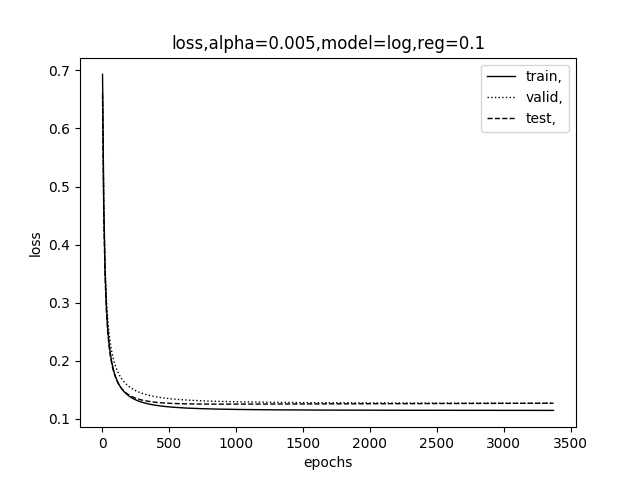
\includegraphics[width=\linewidth]{images/a1/2.2/loss_logistic.png}
\endminipage\hfill
\minipage{0.5\textwidth}
  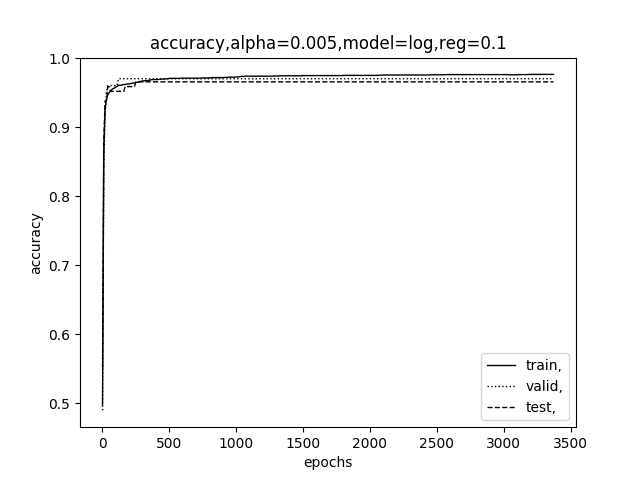
\includegraphics[width=\linewidth]{images/a1/2.2/accuracy_logistic.png}
\endminipage
\caption{Loss (left), Accuracy (right) curves of the logistic regression model using cross entropy loss under settings $\lambda=0.1$, epochs = 5000 and $\alpha=0.005$.}\label{fig:2-2}
\end{figure}


\newpage
\textbf{3. } Figure \ref{fig:2-3} plots the training loss and accuracy behaviour for the logistic regression model using cross entropy loss and the linear regression model using MSE loss, under the settings $\lambda=0$, epochs = 5000 and $\alpha=0.005$. It's observed from the graph that the linear regression model using MSE loss appear to converge faster. Nevertheless, the logistic regression model using cross entropy loss manage to gain higher training accuracy.

\begin{figure}[!htb]
\minipage{0.5\textwidth}
  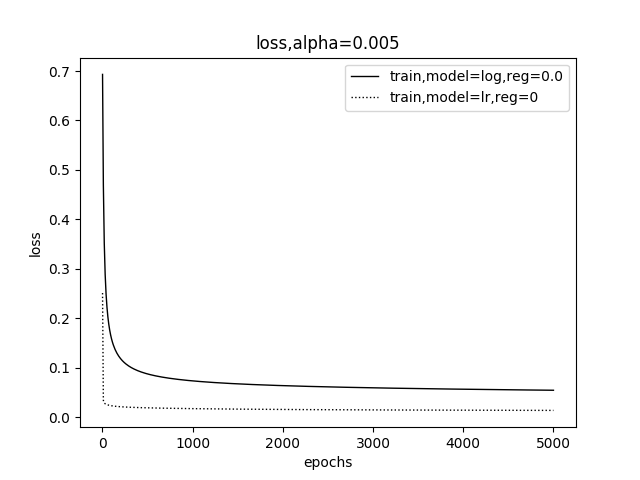
\includegraphics[width=\linewidth]{images/a1/2.3/loss.png}
\endminipage\hfill
\minipage{0.5\textwidth}
  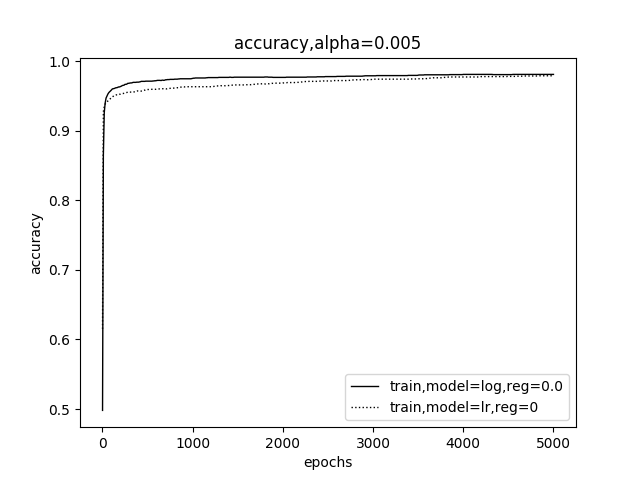
\includegraphics[width=\linewidth]{images/a1/2.3/accuracy.png}
\endminipage
\caption{Traing loss (left), accuracy (right) comparison of the logistic regression model using cross entropy loss (solid line) and the linear regression model with MSE loss (dashed line), under the settings $\lambda=0$, epochs = 5000 and $\alpha=0.005$.}\label{fig:2-3}
\end{figure}
  

\end{problem}

\vspace{5mm}
\newpage
\begin{problem}{3}

\textbf{1. } For simplicity we created a separate file named \texttt{a1-tf.py} for TensorFlow implementions. This file contains SGD algorithm with MSE and Cross Entropy loss, as well as the \texttt{GradientDescentOptimizer} and \texttt{AdamOptimizer}. A code snippet is given below. For more details, refer to the source code.

\begin{lstlisting}[frame=single]
def buildGraph(d, optimizer_type, loss_type, params):
    X = tf.placeholder(tf.float32, shape=(None, d), name='X')
    y = tf.placeholder(tf.float32, shape=(None,), name='y')
    w = tf.Variable(tf.truncated_normal((d,), stddev=0.5), name='w')
    # w = tf.Variable(tf.zeros(d,), tf.float32, name='w')
    reg = tf.placeholder(tf.float32, shape=(), name='reg')

    f = tf.matmul(X, tf.reshape(w, shape=(-1, 1)))
    y_ = tf.reshape(f, shape=(-1,))

    if loss_type == 'mse':
        # loss = tf.losses.mean_squared_error(y, y_)
        loss = tf.reduce_mean(tf.square(y - y_))
    elif loss_type == 'ce':
        loss = tf.losses.sigmoid_cross_entropy(y, y_)
    loss = loss + reg * tf.nn.l2_loss(w[1:])

    if optimizer == 'gd':
        opt_op = tf.train.GradientDescentOptimizer(
            learning_rate=params['alpha'],
        ).minimize(loss)
    else:
        opt_op = tf.train.AdamOptimizer(
            learning_rate=params['alpha'],
            beta1=params['beta1'],
            beta2=params['beta2'],
            epsilon=params['epsilon'],
        ).minimize(loss)

    predict = (tf.sign(y_ - 0.5) + 1) / 2
    accuracy = tf.reduce_mean(tf.cast(tf.equal(y, predict), tf.float32))

    return X, y, y_, w, reg, loss, predict, accuracy, opt_op

\end{lstlisting}

\bigskip

\textbf{2. } The Stochastic Gradient Descent algorithm is implemented to minimize the MSE, under the settings of minibatch size=500, epochs=700, $\alpha=0.001$ and $\lambda=0$. The resulting loss and accuracy curves are presented in figure \ref{fig:3-2}. As seen in the figure, the loss and accuracy curves of the SGD are not as smooth as in the Batch Gradient Algorithm. The overall trend, however, is still to reduce losses and improve accuracy over time. The reason is that each batch update does not reflect the overall gradient, and the accumulation of many updates is what is expected to approximate the effects of overall gradient.

\begin{figure}[!htb]
 \hspace*{-2cm}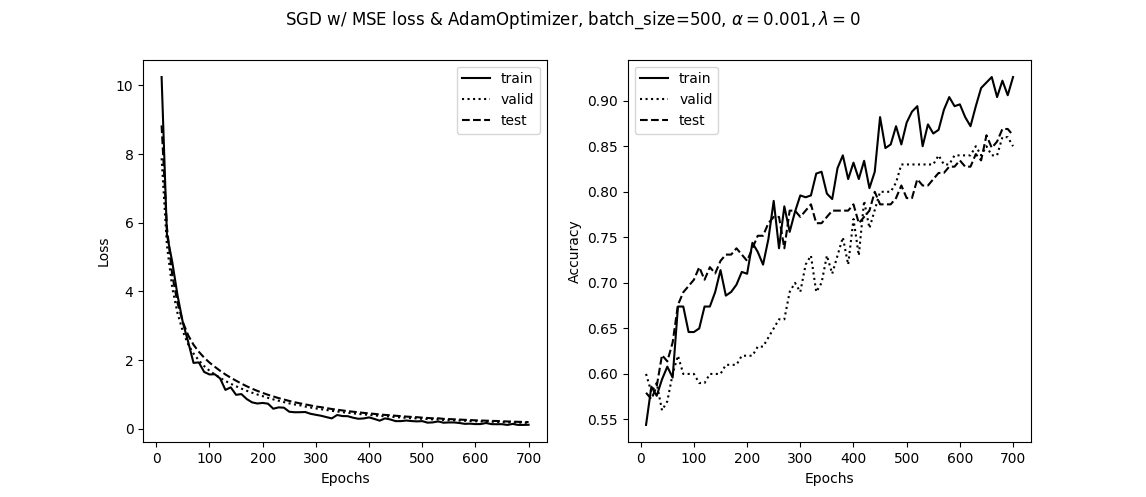
\includegraphics[width=1.2\linewidth]{images/a1/3.2/sgd_loss_accuracy.png}
\caption{SGD algorithm is implemented to minimize the MSE using minibatch size=500 , epochs =700, $\alpha=0.001$ and $\lambda=0$. Training, validation and test loss curves are depicted on the left, with the corresponding accuracy curves on the right.}\label{fig:3-2}
\end{figure}


\bigskip
\newpage
\textbf{3. } To investigate the effects of batch size on the behaviour of the SGD algorithm using Adam, three different batch sizes, namely 100, 700 and 1750 are utilized to plot the loss and accuracy curves in figure \ref{fig:3-3}. Smaller batch size is found to reduce loss and improve accuracy in this case. The rationale for this is that smaller batch size allows for a greater number of updates in each epoch, thus improves the overall performance of the classification.   

\begin{figure}[!htb]
\minipage{0.5\textwidth}
  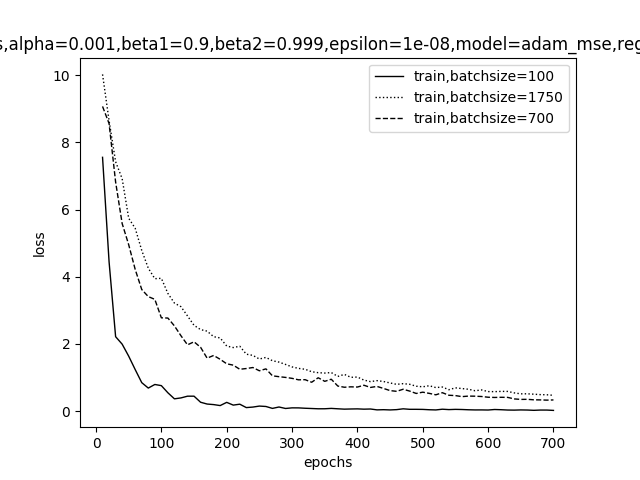
\includegraphics[width=\linewidth]{images/a1/3.3/loss.png}
\endminipage\hfill
\minipage{0.5\textwidth}
  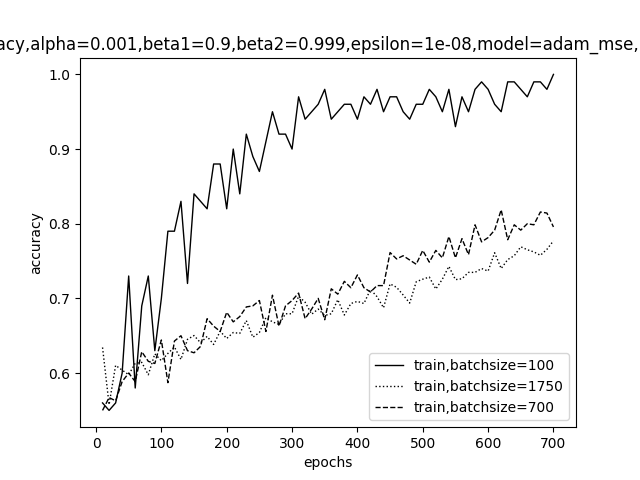
\includegraphics[width=\linewidth]{images/a1/3.3/accuracy.png}
\endminipage

\caption{Three different batch sizes 100, 700, 1750 are used in the SGD algorithm to minimize the MSE. The other settings are epochs =700, $\alpha=0.001$ and $\lambda=0$. Training loss (left) and accuracy (right) curves are plotted.}\label{fig:3-3}
\end{figure}

\bigskip
\bigskip
\bigskip
\textbf{4. } Next we experiment with different values for Adam hyperparameters to investigate their effects on the final training, validation and test accuracy. The minibatch size is set to 500,  $\alpha=0.001$ and epochs=700.

Tensorflow uses the algorithm proposed by Kingma and Ba \cite{adam}. The update rule of the algorithm is listed in Algorithm \ref{alg:adam}.

\begin{algorithm}
    \caption{Adam}
    \label{alg:adam}
    \begin{algorithmic}[1]
        \State{$\theta_0$: initial parameter}
        \State{$m_0 \gets 0$} \Comment{First moment vector}
        \State{$v_0 \gets 0$} \Comment{Second moment vector}
        \State{$t \gets 0$}
        \While{$\theta_t$ not converged}
            \State{$t \gets t + 1$}
            \State{$g_t \gets \nabla_\theta f_t(\theta_{t-1})$}
            \State{$m_t \gets \beta_1\cdot m_{t-1} + (1-\beta_1) \cdot g_t$}
            \State{$v_t \gets \beta_2 \cdot v_{t-1} + (1-\beta_2) \cdot g_t^2$}
            \State{$\alpha_t \gets \alpha \cdot \sqrt{1 - \beta_2^t} / (1 - \beta_1^t)$}
            \State{$\theta_t \gets \theta_{t-1} - \alpha_t \cdot m_t / (\sqrt{v_t} + \epsilon)$}
        \EndWhile
    \end{algorithmic}
\end{algorithm}

\bigskip

(a) $\beta_1 = (0.95, 0.99)$: $\beta_1$ is the exponential decay rate for the first moment estimate. From the update rule $m_t \gets \beta_1\cdot m_{t-1} + (1-\beta_1) \cdot g_t$,  we know that $\beta_1$ controls the weight of first moment (setting $\beta_1=0$ results in regular SGD without moment), and creates a "smoother" gradient than the raw gradient $g_t$.

Table \ref{table:3-4-a} lists the accuracy results from $\beta_1=\{0.95, 0.99\}$ and we can see that there is no significant difference on the final accuracy. Figure \ref{fig:3-4-a} shows the comparison of training loss and accuracy. From the plot we can see that greater $\beta_1=0.99$ has smaller gradient component which results in slightly slower converge.

\begin{table}[!htb]
\center
\begin{tabular}{|l|l|l|l|l|l|}
\hline
$\beta_1$ & training & valid   & test     \\ \hline
0.95      & 92.00\%  & 88.00\% & 88.28\%  \\ \hline
0.99      & 91.60\%  & 87.00\% & 87.59\%  \\ \hline
\end{tabular}
\caption{Comparison of accuracy on $\beta_1=\{0.95, 0.99\}$. Other hyperparameters are $\beta_2=0.999, \epsilon=10^{-8}$.}
\label{table:3-4-a}
\end{table}

\begin{figure}[!htb]
\minipage{0.5\textwidth}
  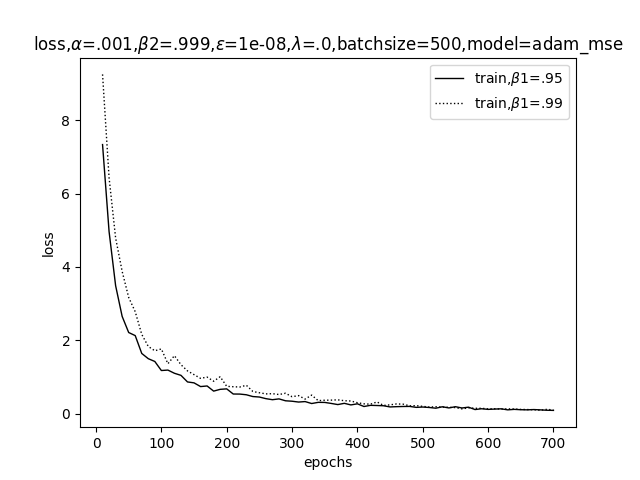
\includegraphics[width=\linewidth]{images/a1/3.4/a/train_loss.png}
\endminipage\hfill
\minipage{0.5\textwidth}
  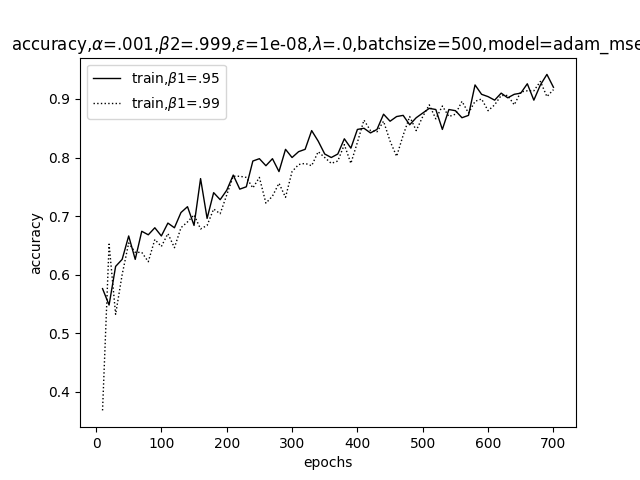
\includegraphics[width=\linewidth]{images/a1/3.4/a/train_accuracy.png}
\endminipage

\caption{Training loss and accuracy for  $\beta1$ = 0.95 and 0.99.
\newline
$\beta_2$ and $\epsilon$ are set to default Tensorflow initialization, batch size=500, $\alpha=0.001$ and epochs=700.  }\label{fig:3-4-a}
\end{figure}

\bigskip
\newpage
(b) $\beta_2 = (0.99, 0.9999)$: $\beta_2$ is the exponential decay rate for the second moment. From $\alpha_t \gets \alpha \cdot \sqrt{1 - \beta_2^t} / (1 - \beta_1^t)$ we know that increasing $\beta_2$ will effectively decrease the learning rate.

Table \ref{table:3-4-b} lists the accuracy on $\beta_2=\{0.99, 0.9999\}$ and we can see that $\beta_2=0.99$ has a higher final accuracy, which indicates $\beta_2=0.99$ converges faster than $\beta_2=0.9999$. Figure \ref{fig:3-4-2} shows the comparison of training loss and accuracy. From the plot we can see that greater $\beta_2=0.9999$ results in slower converge.


\begin{table}[!htb]
\center
\begin{tabular}{|l|l|l|l|l|l|}
\hline
$\beta_2$ & training & valid   & test     \\ \hline
0.99      & 94.20\%  & 90.00\% & 91.03\%  \\ \hline
0.9999    & 86.00\%  & 87.00\% & 80.68\%  \\ \hline
\end{tabular}
\caption{Comparison of accuracy on $\beta_2=\{0.99, 0.9999\}$. Other hyperparameters are $\beta_1=0.9, \epsilon=10^{-8}$.}
\label{table:3-4-b}
\end{table}

\begin{figure}[!htb]
\minipage{0.5\textwidth}
  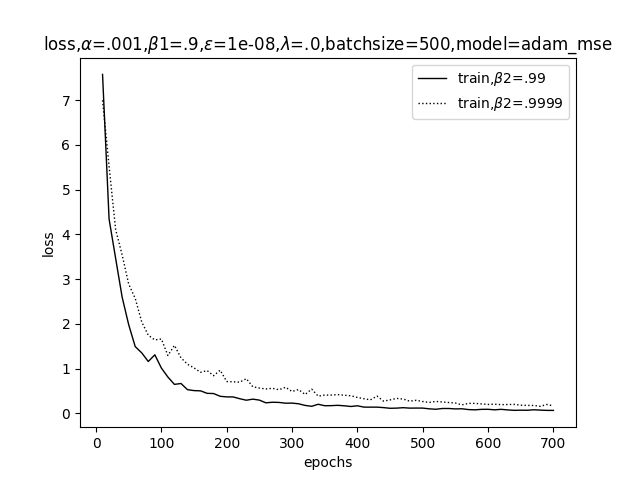
\includegraphics[width=\linewidth]{images/a1/3.4/b/train_loss.png}
\endminipage\hfill
\minipage{0.5\textwidth}
  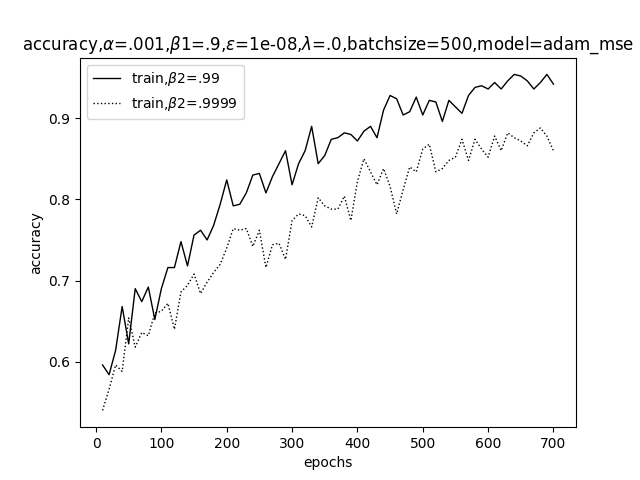
\includegraphics[width=\linewidth]{images/a1/3.4/b/train_accuracy.png}
\endminipage

\caption{Training loss and accuracy for $\beta2$ = 0.99 and 0.9999. 
\newline
$\beta1$ and $\epsilon$ are set to default Tensorflow initialization, batch size=500, $\alpha=0.001$ and epochs=700.  }\label{fig:3-4-2}
\end{figure}

\bigskip
\newpage
(c) $\epsilon = (1e^{-9}, 1e^{-4})$: $\epsilon$ is a small number to avoid zero. However a very small $\epsilon$ results in large weight updates and could potentially result overshooting.

Table \ref{table:3-4-c} lists the accuracy results on $\epsilon=\{10^{-9}, 0.0001\}$ and we can see that $\epsilon=0.0001$ has a higher final accuracy.

\begin{table}[!htb]
\center
\begin{tabular}{|l|l|l|l|l|l|}
\hline
$\epsilon$ & training & valid   & test     \\ \hline
$10^{-9}$   & 89.00\%  & 89.00\% & 82.07\%  \\ \hline
0.0001    & 92.20\%  & 89.00\% & 87.59\%  \\ \hline
\end{tabular}
\caption{Comparison of accuracy on $\epsilon=\{10^{-9}, 0.0001\}$. Other hyperparameters are $\beta_1=0.9, \beta_2=0.999$.}
\label{table:3-4-c}
\end{table}

\newpage
\newpage
\newpage
\bigskip
\bigskip
\bigskip
\bigskip
\newpage
\newpage
\newpage



\textbf{5. } We rerun 3.2 - 3.4 with cross entropy loss function. The final loss and accuracy for different batch size and hyperparameter setting is listed in Table \ref{table:3-5}.

Generally, cross entropy loss meets the analysis we did in 3.2 - 3.4. Overall, however, cross entropy has less loss and higher accuracy than MSE loss at epoch=700, indicating that cross entropy loss converges faster than MSE loss. We may conclude that for binary classification problem, logistic regression with cross entropy loss is a "more suitable" model than linear regression.
 
\begin{table}[!htb]
\center
\begin{tabular}{|l|r|r|r|r|}
\hline
                Optimizer Type and Parameter Value  &       MSE loss &        CE loss &     MSE accuracy &      CE accuracy \\
\hline
       Adam, batch=100 &  0.022417 &  0.001765 & 1.000000 &  1.000000  \\
       Adam, batch=700 &  0.334083 &  0.028498 & 0.795714 &  0.990000 \\
      Adam, batch=1750 &   0.471597 &  0.044727 & 0.777143 &  0.982857  \\
\hline
      Adam, beta1=0.95 &  0.094182 &  0.025064 &0.920000 &  0.990000 \\
      Adam, beta1=0.99 &  0.104681 &  0.025137 & 0.916000 &  0.990000 \\
\hline
      Adam, beta2=0.99 &   0.063865 &  0.011852 & 0.942000 &  0.998000  \\
    Adam, beta2=0.9999 & 0.163707 &  0.035279 &  0.860000 &  0.982000  \\
\hline
    Adam, epsilon=1e-9 &   0.145734 &  0.015310 & 0.890000 &  0.994000 \\
  Adam, epsilon=0.0001 &  0.102104 &  0.024191 & 0.922000 &  0.990000   \\
\hline
\end{tabular}
\caption{Comparison of MSE loss and Cross Entropy loss under different settings, at epoch=700. Data from training loss and training accuracy.}
\label{table:3-5}
\end{table}

\bigskip



\textbf{6. } Figure \ref{fig:3-6} plots the loss and accuracy curves of the SGD and batch gradient descent algorithm for comparison.

SGD does not have a smooth loss curve as Batch GD does. The reason is that each step in SGD considers only a small batch of data for optimizing loss, thus does not guarantee global loss to decrease.

However, SGD converges faster than Batch GD. Table \ref{table:3-6} shows that at epoch=10, SGD converges to loss = 0.0427 while Batch GD still has loss = 0.0924. However at epoch 100 and epoch 500, since SGD cannot guarantee monotonic decreasing of loss, it may have greater loss than Batch GD.

\begin{table}[!htb]
\center
\begin{tabular}{|l|l|l|l|l|l|}
\hline
Epochs & SGD with Adam & Batch GD     \\ \hline
10  & 0.0427 & 0.0924  \\ \hline
100  & 0.0296 & 0.0285  \\ \hline
500  & 0.0261 & 0.0231  \\ \hline
\end{tabular}
\caption{Training loss comparison of Adam SGD vs. Batch GD.}
\label{table:3-6}
\end{table}

\begin{figure}[!htb]
\minipage{0.5\textwidth}
  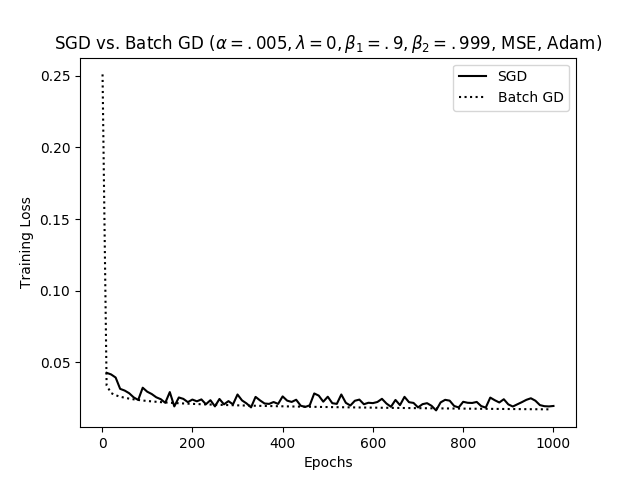
\includegraphics[width=\linewidth]{images/a1/3.6/adam-sgd-vs-bgd-1000epochs-loss.png}
\endminipage\hfill
\minipage{0.5\textwidth}
  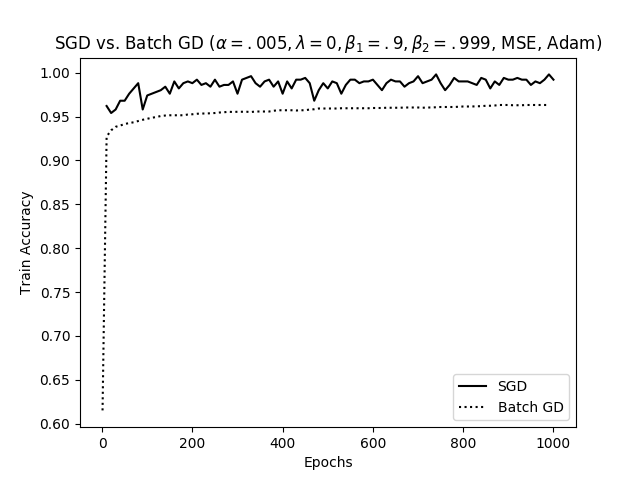
\includegraphics[width=\linewidth]{images/a1/3.6/adam-sgd-vs-bgd-1000epochs-accuracy.png}
\endminipage
\caption{Comparison of SGD with Adam optimizer vs. Batch GD on training loss (left) and training accuracy (right) under the settings $\lambda=0$ and $\alpha=0.005$.}\label{fig:3-6} For comparison, both SGD and Batch GD use zero vector as initial $\textbf{w}$ and $b$ value.
\end{figure}

\end{problem}

\newpage

\begin{thebibliography}{1}
\bibitem{adam} 
Kingma and Ba, 
\textit{Adam: A Method for Stochastic Optimization}. 
https://arxiv.org/abs/1412.6980

\end{thebibliography}

\end{document}